\subsection{Non-Spark Holdout Results: Five Optuna-tuned Models}
\label{subsec:python-optuna-execution}
The completed non-Spark experiment evaluates \textbf{logistic regression, random forest, XGBoost, LightGBM and stacking}. Each uses the same five stratified 70/30 holdouts (seeds 42, 7, 21, 84 and 123), with 223 training and 96 test records per split. RFE retains twenty source fields, continuous predictors receive standardization, and ordinal category codes remain unchanged. Each family receives twenty Optuna trials per seed, evaluated by three-fold training-only ROC--AUC. The selected configuration is refitted on the 223 training records and then predicts the untouched 96-record test partition. No held-out record enters fitting, RFE, scaling or parameter selection. The search spaces and training-CV evidence are documented in Section~\ref{sec:algorithm-selection}.

\begin{table}[H]
\centering\small
\caption{Completed non-Spark Optuna-tuned holdout results: mean and sample SD across five matched seeds, RFE20 and standardization. Highest displayed means are bold.}
\label{tab:holdout-optuna-test}
\begin{tabular}{lrrrrr}
\toprule
Model & AUC & Accuracy & Precision & Recall & F1 \\
\midrule
Logistic regression & \textbf{0.843} $\pm$ 0.037 & 0.754 $\pm$ 0.041 & 0.732 $\pm$ 0.046 & 0.808 $\pm$ 0.071 & 0.766 $\pm$ 0.040 \\
Random forest & 0.803 $\pm$ 0.032 & 0.731 $\pm$ 0.027 & 0.704 $\pm$ 0.034 & 0.804 $\pm$ 0.043 & 0.750 $\pm$ 0.022 \\
XGBoost & 0.793 $\pm$ 0.033 & 0.746 $\pm$ 0.032 & 0.713 $\pm$ 0.027 & \textbf{0.825} $\pm$ 0.062 & 0.764 $\pm$ 0.034 \\
LightGBM & 0.793 $\pm$ 0.015 & 0.723 $\pm$ 0.030 & 0.701 $\pm$ 0.021 & 0.779 $\pm$ 0.079 & 0.736 $\pm$ 0.040 \\
Stacking & 0.824 $\pm$ 0.038 & \textbf{0.762} $\pm$ 0.039 & \textbf{0.740} $\pm$ 0.044 & 0.812 $\pm$ 0.042 & \textbf{0.774} $\pm$ 0.034 \\
\bottomrule
\end{tabular}
\end{table}


Table~\ref{tab:holdout-optuna-test} contains \textbf{test results}, not the training-CV scores shown in Section 6.1. It summarises twenty-five completed tuned model/seed evaluations from \path{results/holdout/metrics_per_seed.csv}, with fitted pipelines, predictions, best parameters and trial traces retained per model. Mean and sample standard deviation describe the five split-specific outcomes. The partitions overlap, so this variation is not independent cohort replication. Metrics use gallstones-present class 1 and a probability threshold of 0.5.

Among the five Optuna-tuned candidates, logistic regression has the highest mean test AUC (0.843). Stacking has the highest mean accuracy (0.762), while XGBoost has the highest mean recall (0.825). These are metric-specific observations rather than an overall ranking: discrimination, false negatives and false positives need to be considered together. Both project targets (AUC $\geq0.80$ and recall $\geq0.80$) were met in two of five splits for logistic regression, random forest and LightGBM, and three of five for XGBoost and stacking. Training-CV selection and observed test performance can therefore favour different families without contradicting the evaluation procedure.

\begin{figure}[H]
\centering
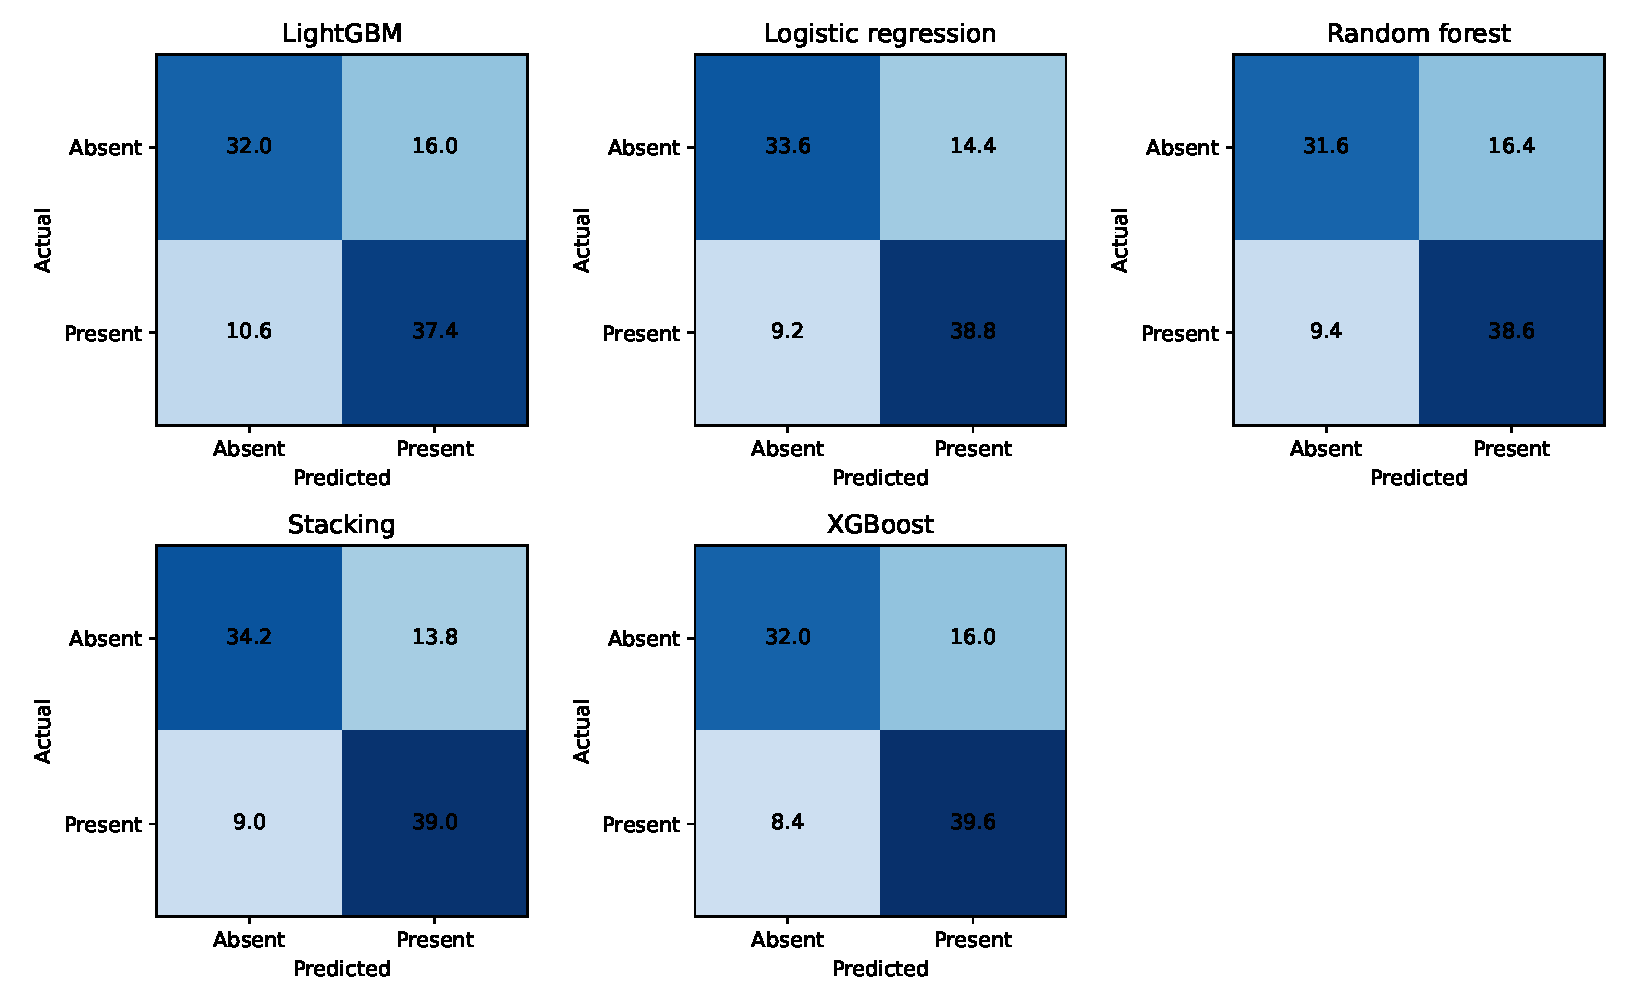
\includegraphics[width=.85\textwidth]{figures/modeling/holdout_average_cm.pdf}
\caption{Average non-Spark test confusion counts across five holdouts for each Optuna-tuned family. Fractional counts arise from averaging 96-record test sets.}
\end{figure}

\subsection{Non-Spark Fixed-parameter Holdout Reference}
The following fixed-model reference uses the same RFE20 preparation and test memberships. It supports comparison with the tuned procedure without mixing fixed and tuned rows in the main Optuna result table. The training-prior dummy is included as a baseline; its perfect recall is obtained by predicting every record as positive and is accompanied by zero specificity.

\begin{table}[H]
\centering\small
\caption{Non-Spark fixed-parameter holdout reference: RFE20 and standardization with the same five test partitions. Highest displayed means are bold, including ties and the prior dummy.}
\label{tab:holdout-fixed-test}
\begin{tabular}{lrrrr}
\toprule
Model & AUC & Recall & Specificity & Accuracy \\
\midrule
Logistic regression & \textbf{0.832} $\pm$ 0.042 & 0.817 $\pm$ 0.063 & 0.688 $\pm$ 0.081 & \textbf{0.752} $\pm$ 0.046 \\
Random forest & 0.808 $\pm$ 0.047 & 0.783 $\pm$ 0.041 & 0.700 $\pm$ 0.075 & 0.742 $\pm$ 0.041 \\
XGBoost & 0.801 $\pm$ 0.030 & 0.796 $\pm$ 0.073 & 0.688 $\pm$ 0.042 & 0.742 $\pm$ 0.032 \\
LightGBM & 0.799 $\pm$ 0.027 & 0.775 $\pm$ 0.063 & 0.679 $\pm$ 0.035 & 0.727 $\pm$ 0.028 \\
Stacking & 0.824 $\pm$ 0.029 & 0.787 $\pm$ 0.048 & \textbf{0.708} $\pm$ 0.074 & 0.748 $\pm$ 0.017 \\
Prior dummy & 0.500 $\pm$ 0.000 & \textbf{1.000} $\pm$ 0.000 & 0.000 $\pm$ 0.000 & 0.500 $\pm$ 0.000 \\
\bottomrule
\end{tabular}
\end{table}


The controlled scaling, selector and feature-count comparisons are interpreted in Section~\ref{sec:multiple-iteration}. The full saved outputs additionally contain specificity, balanced accuracy, false-negative rate, log loss, fit/prediction time and other metrics. A larger search is not assumed to improve every model; its effect is judged against the matched fixed reference.

\subsection{Native Spark Holdout Results in Google Colab}
The native Spark execution provides a separate platform-based holdout evaluation using PySpark for loading, preparation, model fitting, training-only cross-validation, predictions and metrics. The latest completed Colab holdout output retrieved from the shared Google Drive folder trained native Spark logistic regression, random forest and gradient-boosted trees on five stratified 70/30 holdouts (seeds 42, 7, 21, 84 and 123). Each split used 223 training and 96 test records. All 38 source fields were retained; continuous fields were standardized and original ordinal codes were preserved. Three-fold Spark CrossValidator operated on training records only.

\begin{table}[H]
\centering\small
\caption{Completed native PySpark holdout results from Google Drive: mean and sample SD across five seeds. Highest displayed metric means and lowest error rate are bold; ties share highlighting.}
\label{tab:spark-colab-execution}
\resizebox{\textwidth}{!}{\begin{tabular}{lrrrrrrr}
\toprule
Model & AUC & Accuracy & Precision & Recall & Specificity & F1 & Error rate \\
\midrule
Spark GBT & 0.804 $\pm$ 0.045 & 0.721 $\pm$ 0.056 & 0.701 $\pm$ 0.057 & 0.779 $\pm$ 0.043 & 0.662 $\pm$ 0.092 & 0.737 $\pm$ 0.044 & 0.279 $\pm$ 0.056 \\
Logistic regression & \textbf{0.873} $\pm$ 0.027 & \textbf{0.810} $\pm$ 0.029 & \textbf{0.766} $\pm$ 0.042 & \textbf{0.900} $\pm$ 0.040 & \textbf{0.721} $\pm$ 0.072 & \textbf{0.826} $\pm$ 0.023 & \textbf{0.190} $\pm$ 0.029 \\
Random forest & 0.806 $\pm$ 0.056 & 0.715 $\pm$ 0.052 & 0.714 $\pm$ 0.044 & 0.713 $\pm$ 0.081 & 0.717 $\pm$ 0.041 & 0.713 $\pm$ 0.060 & 0.285 $\pm$ 0.052 \\
\bottomrule
\end{tabular}}
\end{table}
All metrics describe the same three models and five 96-record test holdouts, using the full-precision completed Drive output dated 12 October 2026. Recall is sensitivity; error rate equals one minus accuracy. Precision and F1 measure different properties, so their values need not equal accuracy or AUC. These test metrics are separate from training-CV selection evidence.


Table~\ref{tab:spark-colab-execution} consolidates all Spark test metrics from one experiment. The raw output was saved on 12 October 2026 and contains fifteen complete model/seed evaluations. Its full-precision metric file, source notebook invocation and provenance are retained in \path{results/spark_holdout_drive}. Bold entries identify the highest displayed means within each metric column, with ties highlighted together; error rate is minimized. Standard deviations are reported rather than ranked.

The saved execution demonstrates actual use of Spark and Colab, while the GitHub repository supplies the source and saved notebook evidence. It does not establish that the newer CART20/RFE20/RFE10 extension has already run. Its pipeline performs selection within native Spark fits and records the corresponding tuning traces when executed. Spark GBT is a separate implementation from XGBoost and LightGBM.

\begin{figure}[H]
\centering
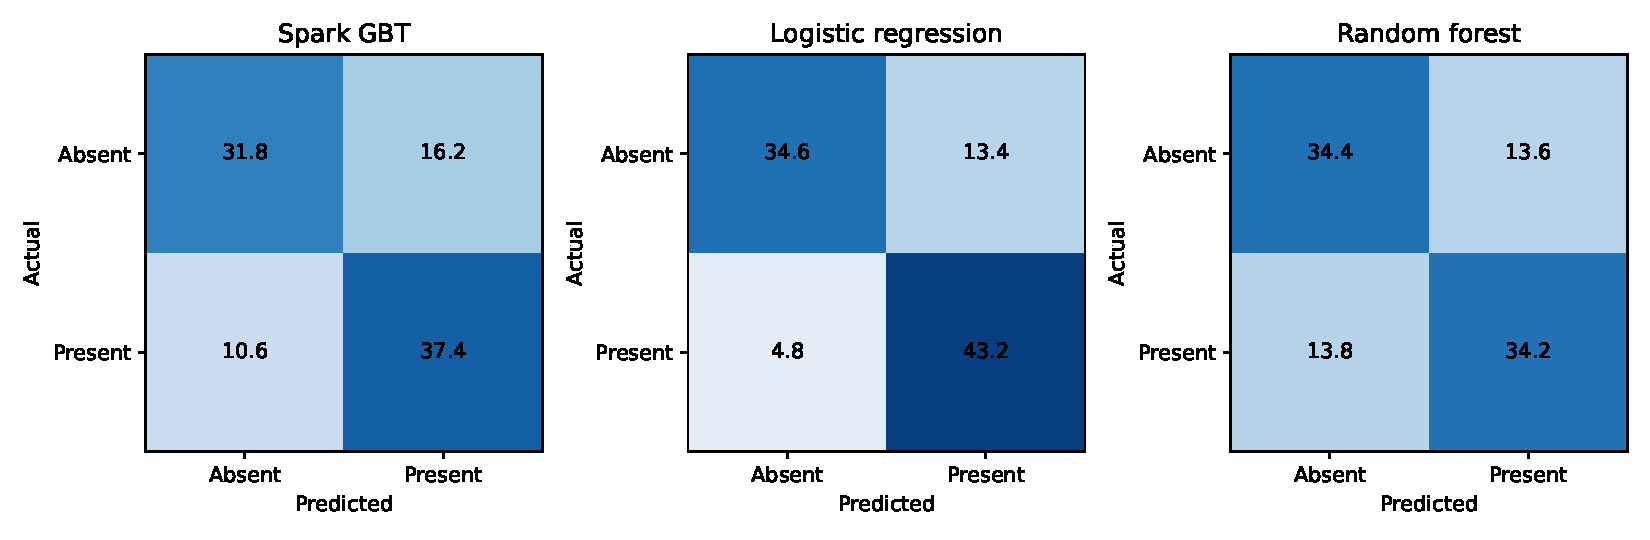
\includegraphics[width=.95\textwidth]{figures/modeling/spark_average_cm.pdf}
\caption{Mean native Spark test confusion counts over the latest five completed Google Drive holdouts. Counts are averaged rather than pooled into an independent new cohort.}
\end{figure}


The native Spark results use all thirty-eight predictors and Spark estimators, whereas the non-Spark Optuna results above use RFE20 and their Python estimator implementations. They demonstrate the two completed workflows; a numerical difference between them cannot be attributed to Spark alone. No LOPO scores are included in these holdout tables.
